
%%%%%%%%%%%%%%%%%%%%%%% file typeinst.tex %%%%%%%%%%%%%%%%%%%%%%%%%
%
% This is the LaTeX source for the instructions to authors using
% the LaTeX document class 'llncs.cls' for contributions to
% the Lecture Notes in Computer Sciences series.
% http://www.springer.com/lncs       Springer Heidelberg 2006/05/04
%
% It may be used as a template for your own input - copy it
% to a new file with a new name and use it as the basis
% for your article.
%
% NB: the document class 'llncs' has its own and detailed documentation, see
% ftp://ftp.springer.de/data/pubftp/pub/tex/latex/llncs/latex2e/llncsdoc.pdf
%
%%%%%%%%%%%%%%%%%%%%%%%%%%%%%%%%%%%%%%%%%%%%%%%%%%%%%%%%%%%%%%%%%%%


\documentclass[runningheads,a4paper]{llncs}

\usepackage{amssymb}
\setcounter{tocdepth}{3}
\usepackage{graphicx}
\usepackage{bm}
\usepackage{multirow}

%\usepackage{url}
%\urldef{\mailsa}\path|{alfred.hofmann, ursula.barth, ingrid.haas, frank.holzwarth,|
%\urldef{\mailsb}\path|anna.kramer, leonie.kunz, christine.reiss, nicole.sator,|
%\urldef{\mailsc}\path|erika.siebert-cole, peter.strasser, lncs}@springer.com|    

\newcommand{\keywords}[1]{\par\addvspace\baselineskip
\noindent\keywordname\enspace\ignorespaces#1}

\begin{document}

\mainmatter  % start of an individual contribution

% first the title is needed
\title{Samsung!}

% a short form should be given in case it is too long for the running head
\titlerunning{Samsung!}


%\thanks{Please note that the LNCS Editorial assumes that all authors have used
%the western naming convention, with given names preceding surnames. This determines
%the structure of the names in the running heads and the author index.}%

% the name(s) of the author(s) follow(s) next
\author{Darya Lavrova, Ruslan Gaisin, Iskander Kareev, Rustem Salimov}
%
\authorrunning{Author running}
% (feature abused for this document to repeat the title also on left hand pages)

% the affiliations are given next; don't give your e-mail address
% unless you accept that it will be published
\institute{Kazan Federal University}
%Springer-Verlag, Computer Science Editorial,\\
%Tiergartenstr. 17, 69121 Heidelberg, Germany\\
%\mailsa\\
%\mailsb\\
%\mailsc\\
%\url{http://www.springer.com/lncs}}

%
% NB: a more complex sample for affiliations and the mapping to the
% corresponding authors can be found in the file "llncs.dem"
% (search for the string "\mainmatter" where a contribution starts).
% "llncs.dem" accompanies the document class "llncs.cls".
%

\toctitle{toc title}
\tocauthor{toc author}
\maketitle


\begin{abstract}
Abstract
\keywords{keywords}
\end{abstract}


\section{Introduction}



\section{Demographic Clusterisation of the Gathered Data}


The investigation was done on the basis of dataset consisting of user's age $x_1$ (column \textit{webapi\_agecateg}), gender $x_2$ (\textit{gender}), marital status $x_3$ (\textit{marital}), occupational status $x_4$ (\textit{jposition}) and infomation on their Internet activity --- the urls which they have visited. 

To improve the robustness of the investigation and clearness of its results we have excluded the urls which were visited with less than 5 users. After the we had total of 526 user entries and 316000 entries on url visits.

Put $U$ to be the set of all users, $S$ to be the set of all sites (urls). By $S(A)$ denote the set of all sites which were visited by at least one user $u \in A \subseteq U$. By $U(s)$ denote the set of all users which visited the site $s \in S$.



\subsection{Clusterization of Users by Demographic Attributes with Control on Diversification of Derived URLs Sets}



On this part of the investigation we have recoded the values in the following way:
\begin{itemize}
\item for values of \textit{marital}: \\ 
	``\textit{Single}''  $\to$ 0,  \quad  ``\textit{In relations}''  $\to$ 0.5, \quad  ``\textit{Married}''  $\to$ 1;
\item for values of \textit{gender}: \\ 
	``\textit{Male}''  $\to$ 0, \quad  ``\textit{Female}'' $\to$ 1;
\item for values of \textit{webapi\_agecateg}: \\ 
	``\textit{0..17}''  $\to$ 1, \quad  ``\textit{18..24}''  $\to$ 2, \quad     ``\textit{25..34}''  $\to$ 3, \quad  ``\textit{35..44}''  $\to$ 4, \quad     ``\textit{45+}''  $\to$ 5;
\item for values of \textit{jposition}: \\ 
	``\textit{employee}'' $\to$ 1, \quad  ``\textit{executive}'' $\to$ 1, \quad  ``\textit{jobless}'' $\to$ 0, \quad  ``\textit{minor}'' $\to$ 0, \quad  ``\textit{student}'' $\to$ 0.5.
\end{itemize}

This allows easy application of classic clusterisation algorithms based on Euclid distance. Here we apply the hierarchic algorithm. The results of clusterisation are highly dependant on the scale of the variables. That is why all the variables were scaled by their means and variances. We bring in a vector of coefficients $\boldsymbol{w} = (w_1, w_2, w_3, w_4), \quad w_i \in [0, 1]$, so rescaled values are supplied to the clusterisation algorithm of the form:
\[
	(w_1 x_1, w_2 x_2, w_3 x_3, w_4 x_4).
\]


\subsubsection{Sites separation measure.}

Let us describe the considered way of choosing of coefficients $\boldsymbol{w}$ values.

Suppose that after the clusterisation with some $\boldsymbol{w}$ the users $U$ are divided on $k$ sets $C_1, C_2, \dots, C_k$:
\[
	C_1 + C_2 + \dots + C_k = U.
\]
Let
\[
	r_{s,j} = \frac{\mathcal{N}(U(s) \cap C_j)}{\mathcal{N}(C_j)}.
\]
By means of $r_{s,j}$ we define an intersection measure for the clusterisation $C_1, C_2, \dots, C_k$:
\[
	M_I(\boldsymbol{w}) = \sum_s \Big( \sum_j r_{s,j} - \min_j \{r_{s,j}\} \Big).
\]

For given number of clusters $k$ we choose the weights $\boldsymbol{w}$ as the ones for which $I(\boldsymbol{w})$ is minimized.



\subsubsection{Clusters number.}

Let $M_I(k) = \min_w M_I(k, \boldsymbol{w})$ be the intersection measure for clustering into $k$ clusters. Fig. illustrates the dependance of the number of unique sites in each group and the value of $M_I$ on value of $k$.

\begin{figure}\label{N7Jti}

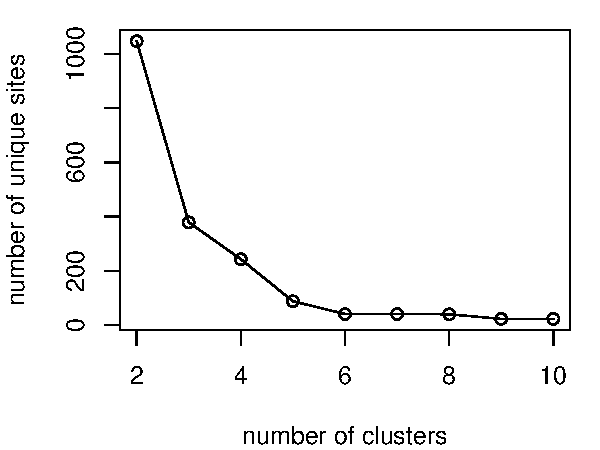
\includegraphics[scale=0.6]{fig_uurls.pdf}\hfill
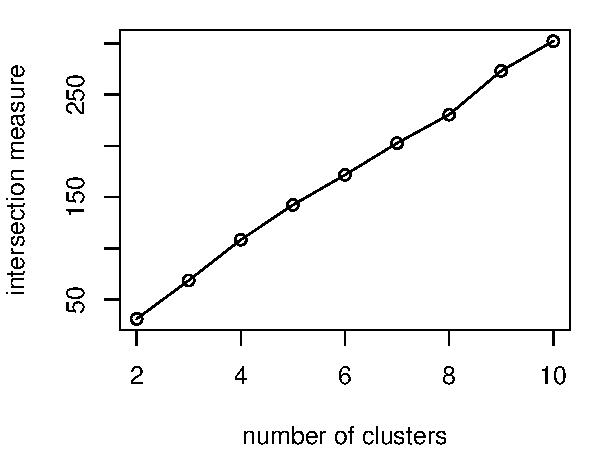
\includegraphics[scale=0.6]{fig_meas.pdf}

\caption{tru-la-la}
\end{figure}

After the AIC algorithm results we chose $k=6$ as the clusters number. For this the weights minimizing the interception measure $M_I$:
\[
	\boldsymbol{w} = (0.4, 0.4, 1.0, 0.4).
\]
On that values of weights we might suggest that the age (to which correspond the weight $1.0$) has the most has the most distinguishing effect on the visiting Internet sites.


\subsubsection{The results.}



\begin{table}\label{OWoti}
	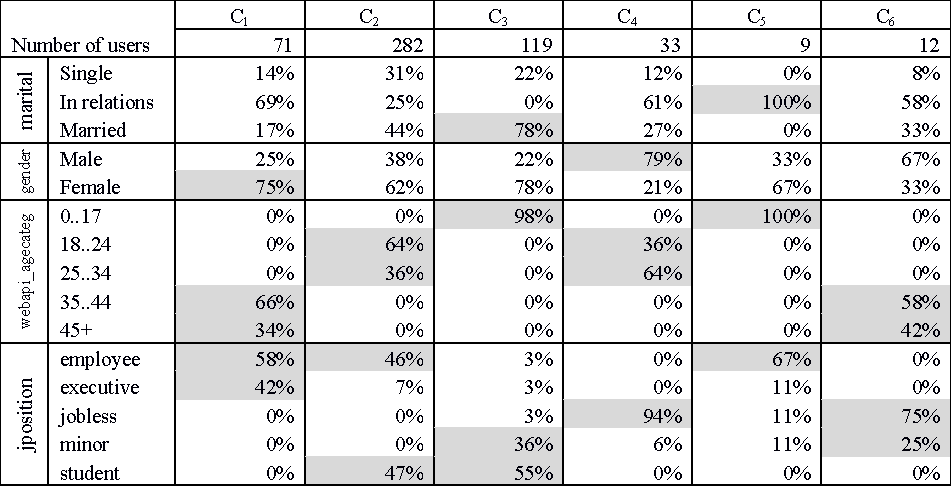
\includegraphics[width=\linewidth]{t1.pdf}
	
	\caption{asd}
\end{table}



\begin{table}\label{01Yti}
	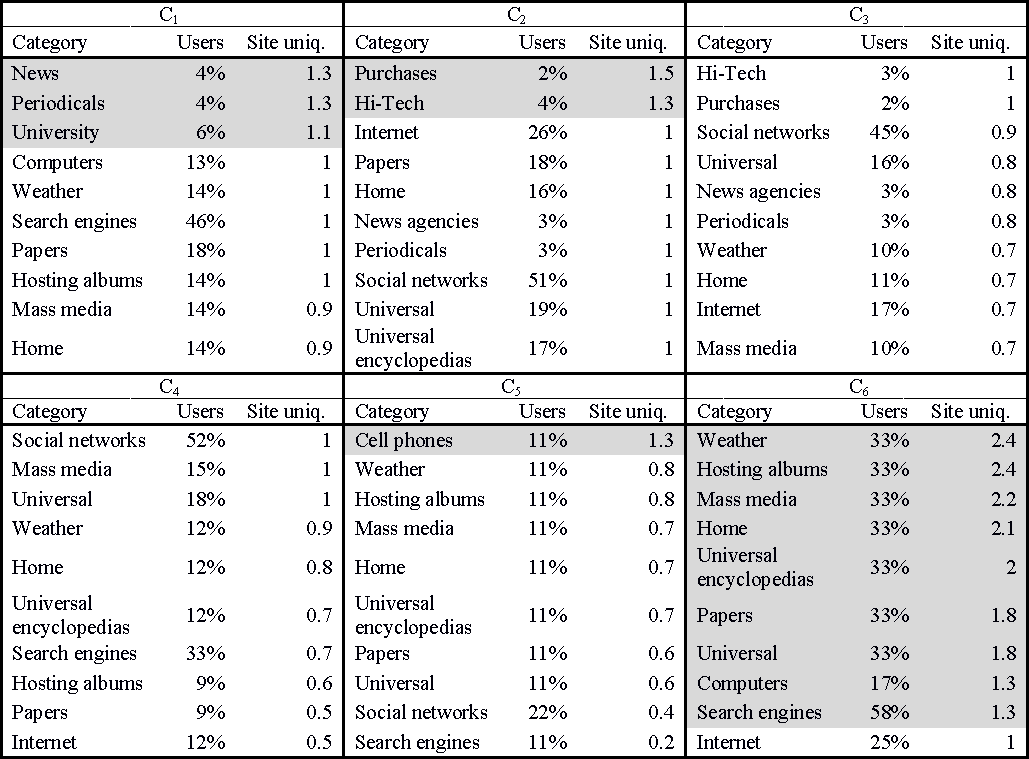
\includegraphics[width=\linewidth]{t2.pdf}
	
	\caption{asd}
\end{table}



\section{Dependency analysis of attributes and sites visits}

One of the problems was the task of checking the independence of the attributes of the data and sites categories. For this purpose chi-squared test is usually used if explored indications are qualitative (see: \cite{wiki_chisq}). So we had to build a contingency tables and to make decisions about hypothesis of independence.

Originally it was planned to analyze the relationships between the features of respondents and visits to the sites. However, for most sites this version of the analysis is not suitable due to the fact that they have a small number of visits; the same time for the sites with big number of visits(vk.com, google.com, and so on) to allocate a significant relationship is not possible. Therefore, it was decided to group the original sites into categories for further analyzing. The categories with large number of visits (more than 1000) were selected for the analysis, because for the categories with fewer visits the study is not applicable due to the limitations of test. For each user and each category has been allocated fact of the visit (variable that possesses values 0 or 1). After that contingency tables were built and by these tables the hypotheses of independence were tested with a significance level 0.05.

It should be noted that two most popular categories: "Social networks", "Bots" - in which the number of visits by much more than in all other categories, depending on the features of the respondents users could not be found. That is a logical result, because websites of the most popular categories should be visited by users regardless of age, sex and other features. 

A little bit strange result is that a visit to any one of the categories doesn’t depend on the gender of the respondents. Perhaps this is due to a not enough large sample size.

Some interesting relations:

\begin{itemize}
	\item Between the \textbf{age} attribute and the category "\textbf{Newspapers}" (with a high significance level 0.0015) The result shows the benefit of young people aged 0 to 24 years of age and older people 45+ are much more likely not visit sites category "Newspapers".
	\item Between the \textbf{marital status} and the category "\textbf{Dating}" (the significance level of 0.026). As expected, unmarried single people visit sites "dating" category.
	\item Between the \textbf{age} attribute and category of websites "\textbf{Dating}" (with a high level of significance 0.009). Older people visit dating sites are more likely than younger ones.
	\item Between the \textbf{age} attribute and the "Internet" category (with a high level of significance 0.01). It confirms the assumption that young people are more likely to visit sites with such a category.
	\item Between the \textbf{age} attribute and category of "\textbf{Information Agency}" (with a significance level of 0.022). Here we see an unclear relation: young people under the age of 17 years, significantly more likely to visit sites with the category News agencies.
	\item Between marital status and the category "\textbf{Shopping}" (a high level of importance of 0.0053). Married people, or irrelevant, significantly more likely to visit sites category Shopping, in turn, single people opposite.
	\item Between the \textbf{age} attribute and the category of websites "Work" (the significance level of 0.013). Young people were significantly more interested in work sites category.
	\item Between the \textbf{age} attribute and the category "\textbf{Universal Encyclopedia}" (high significance level 0.0023). Young people between 18 and 24 years old visit sites og the category "Universal Encyclopedia" rare than younger participants (0..17) and slightly older participants (24..34).
	\item Between the \textbf{workplace} and the category "\textbf{Universal Encyclopedia}" (high significance level 0.0082). For this feature the obvious relation that students use the sites of this category more often than other groups figured out again. Complete workers also use sites of this category.
	\item Between the \textbf{age} attribute and the category "\textbf{Humor}" (significance level 0.04). For this category we get the obvious connection that young people aged 18 to 34 years visited sites category humor more often.
	\item Between the \textbf{labor} attribute and category of websites "\textbf{Humor}" (significance level 0.03). The connection that students visit sites in this category more often is highlighted here.
\end{itemize}



\subsubsection*{Acknowledgments.} The heading should be treated as a
subsubsection heading and should not be assigned a number.

\begin{thebibliography}{4}

\bibitem{wiki_chisq} Wikipedia: Chi-Square Test  \url{https://en.wikipedia.org/wiki/Chi-squared\_test}

\end{thebibliography}




\end{document}
